\documentclass[10pt]{article}
\usepackage{icmlko}

\icmlmeta{IP 파운데이션 월드모델}{52}{축은 설명하지 않아도 정렬한다}{단독 상관을 세 배로 키워도 전체가 안 오르는데 아예 끄면 크게 떨어진다 --- 이 축은 다른 일을 하고 있었다}

\begin{document}

\twocolumn[
\icmlheader

\begin{abstract}
노트 51이 펀딩 창작자 이력을 건수에서 최대 후원자 수로 바꿔 $-$0.018을
$+$0.180으로 만들었다. 그러면 노트 50의 여섯 도메인 비교가 불공정하므로 나머지도
같은 눈금으로 다시 쟀다. \textbf{넷 중 셋에서 최대 규모가 건수를 2--3배 이긴다}
--- 도서 $+$0.030$\to+$0.091, 게임 $+$0.089$\to+$0.176, 펀딩
$-$0.018$\to+$0.180. \textbf{노트 50의 ``이력이 통하는 시장과 통하지 않는
시장''을 완전히 철회한다} --- 측정 방식 차이를 시장 성질로 오독한 것이었다.
그런데 축으로 켜니 서른 셀 평균이 $+$0.0005에서 $+$0.0021밖에 안 움직인다.
단독 상관을 세 배로 키웠는데 전체는 꿈쩍하지 않는다. 그래서 반대로 물었다 ---
\textbf{아예 끄면?} 매장 노출도를 여섯 도메인에서 전부 끄자 $-$0.0312,
웹툰만 꺼도 $-$0.0248이다. \textbf{축의 가치가 라벨 설명력이 아니라 다른 데
있다.} 공통 축이 셋이면 쌍별 프로크루스테스가 $3\times2$ 적재를 맞추고 둘이면
$2\times2$를 맞춘다. 매장 노출도는 라벨을 잘 설명해서가 아니라 \textbf{정렬에
쓸 세 번째 축을 제공해서} 값을 한다. 그래서 그 축의 내용을 개선해도 전체가
안 오르고, 없애면 크게 떨어진다.
\end{abstract}
]

\section{같은 눈금으로 다시 쟀다}

노트 51의 발견 --- 펀딩 이력은 \emph{몇 번 했느냐}가 아니라 \emph{가장 크게
닿은 것이 얼마나 컸느냐} --- 을 나머지 도메인에 적용했다.

\begin{figure}[t]
\centering
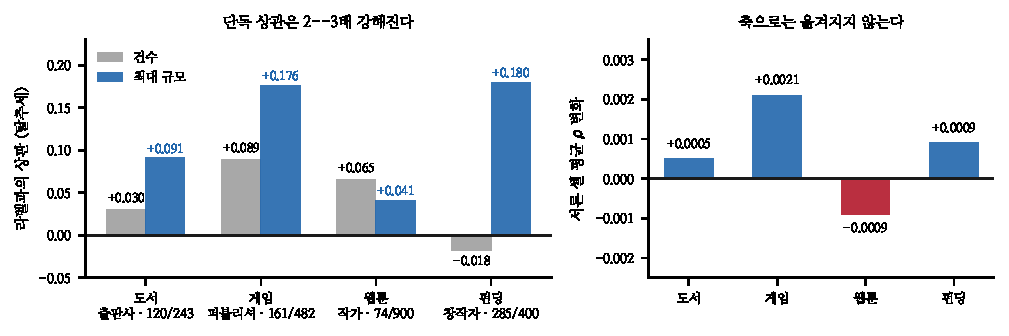
\includegraphics[width=\textwidth]{figs/maxprior.pdf}
\caption{왼쪽 --- 단독 상관. 오른쪽 --- 축으로 켰을 때의 전체 변화.}
\end{figure}

\begin{table}[t]
\centering\tsize
\caption{사전 이력을 두 방식으로.}
\begin{tabular}{llrrr}
\toprule
도메인 & 주체 & 이력 있는 것 & 건수 & 최대 규모 \\
\midrule
펀딩 & 창작자 & 285/400 & $-$0.018 & \textbf{$+$0.180} \\
게임 & 퍼블리셔 & 161/482 & $+$0.089 & \textbf{$+$0.176} \\
도서 & 출판사 & 120/243 & $+$0.030 & \textbf{$+$0.091} \\
웹툰 & 작가 & 74/900 & $+$0.065 & $+$0.041 \\
\bottomrule
\end{tabular}
\end{table}

\claimx{사전 이력은 건수가 아니라 최대 규모로 재야 한다. 넷 중 셋에서 2--3배
강해진다.}{웹툰이 예외인데 이력 있는 것이 74/900뿐이다. 표본을 늘려도 예외로
남으면 도메인 성질이다.}

\paragraph{노트 50을 완전히 철회한다}
그 노트는 여섯 도메인의 매장 노출도 신호를 나란히 놓고($+$0.322에서
$-$0.011까지) ``이력이 통하는 시장과 통하지 않는 시장''이라고 읽었다. 다섯
도메인이 전부 건수로 잰 값이었으므로 그 비교는 성립하지 않는다.
\textbf{시장 성질이 아니라 측정 방식 차이였다.}

\paragraph{아이돌은 잴 수 없었다}
소속사가 68개인데 2건 이상이 5개뿐이라 사전 이력이 거의 없다. 게다가
`SM'과 `SM엔터테인먼트'가 따로 세어진다 --- 정규화가 빠져 있다. 표본 81건에
주체 68개면 노트 40의 펀딩과 같은 희소성 문제이며, 정규화를 고쳐도 크게
달라지지 않을 것이다.

\section{그런데 축으로는 안 옮겨진다}

\begin{table}[t]
\centering\tsize
\caption{최대 규모를 매장 노출도 축으로 켠 결과. 현행 $\rho=+0.3447$.}
\begin{tabular}{lrrr}
\toprule
도메인 & 전체 $\Delta$ & 대상 & 출처 \\
\midrule
게임 & $+$0.0021 & $+$0.346$\to+$0.348 & $+$0.342$\to+$0.352 \\
펀딩 & $+$0.0009 & $+$0.214$\to+$0.262 & $+$0.385$\to+$0.342 \\
도서 & $+$0.0005 & $+$0.224$\to+$0.227 & $+$0.367$\to+$0.367 \\
웹툰 & $-$0.0009 & $+$0.375$\to+$0.381 & $+$0.314$\to+$0.304 \\
\bottomrule
\end{tabular}
\end{table}

단독 상관을 세 배로 키웠는데 전체는 소수점 셋째 자리에서만 움직인다.
\textbf{상충이 항상 나타나는 것도 아니다} --- 노트 51의 펀딩은 대상 $+$0.048에
출처 $-$0.043으로 정확히 상쇄됐는데, 게임은 대상과 출처가 \emph{둘 다} 오른다.
노트 51의 ``정확한 상쇄''는 일반 법칙이 아니라 그 사례의 성질이었다.

\section{아예 끄면 크게 떨어진다}

반대 방향으로 물었다.

\begin{figure}[t]
\centering
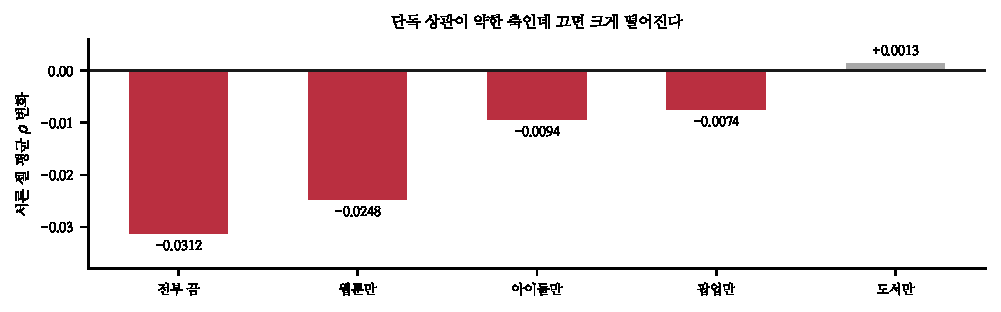
\includegraphics[width=\textwidth]{figs/venueoff.pdf}
\caption{매장 노출도를 끌 때의 손해.}
\end{figure}

\begin{table}[t]
\centering\tsize
\caption{매장 노출도 축을 끄면.}
\begin{tabular}{lr}
\toprule
& 서른 셀 평균 $\rho$ 변화 \\
\midrule
\textbf{여섯 도메인 전부 끔} & \textbf{$-$0.0312} \\
웹툰만 끔 & $-$0.0248 \\
아이돌만 끔 & $-$0.0094 \\
팝업만 끔 & $-$0.0074 \\
도서만 끔 & $+$0.0013 \\
\bottomrule
\end{tabular}
\end{table}

내용을 세 배 좋게 해도 $+$0.002인데 없애면 $-$0.031이다. 그리고 가장 크게
떨어지는 것이 \textbf{웹툰}인데, 웹툰의 매장 노출도는 표본 내 SD가 0.13으로
가장 약한 축이다(노트 46에서 상수 강등 문턱을 겨우 넘었다).

\claimx{공통 축의 가치는 두 종류다 --- 라벨을 설명하는 몫과 정렬에 쓰이는 몫.
매장 노출도는 앞의 것이 약하고 뒤의 것으로 값을 한다. 공통 축이 셋이면 쌍별
프로크루스테스가 $3\times2$ 적재를 맞추고 둘이면 $2\times2$를 맞추는데, 그
차이가 축 내용보다 크다.}{정렬 자유도가 이유라면 아무 값이나 넣어도(잡음이라도)
축을 켜는 것만으로 회복돼야 한다. 잡음 축으로 시험하면 이 설명을 직접 검정할
수 있다.}

이것이 여러 노트에 흩어져 있던 조각을 묶는다.

\begin{itemize}[leftmargin=1.1em,itemsep=0.15em]
\item 노트 37이 공통 축을 둘에서 셋으로 늘려 얻은 것($+$0.0215)이 축 내용이
      아니라 자유도였다.
\item 노트 43에서 게임 매장 노출도를 껐을 때 게임 대상 셀만 좋아진 것도
      --- 게임은 그 축을 관측하지 못하므로 다른 도메인과 두 축으로 정렬한다 ---
      자유도 이야기다.
\item 노트 51에서 펀딩 이력을 개선해도 전체가 안 움직인 것이 여기서 설명된다.
      축은 이미 켜져 있었고 내용만 바뀌었다.
\end{itemize}

\section{한계}

\begin{itemize}[leftmargin=1.1em,itemsep=0.15em]
\item ``정렬 자유도'' 설명을 잡음 축으로 검정하지 않았다. 반증 조건에 적었고
      다음에 한다.
\item 전부 끔의 짝지은 구간이 $[-0.051,\ +0.024]$로 0을 포함한다(P$=$0.085).
      방향은 뚜렷하지만 확정은 아니다.
\item 아이돌 소속사 정규화 결함을 발견만 하고 고치지 않았다.
\item 최대 규모는 그 도메인의 \emph{과거 라벨}을 쓴다. ``대상 라벨을 한 번도
      보지 않는 전이''라는 원칙에서 한 걸음 물러선 것이며, 실무적으로는 예측
      시점에 관측 가능하므로 문제가 없다고 보았다. 그 판단을 따로 검토하지 않았다.
\item 웹툰이 예외인 이유를 표본 부족으로만 설명했다.
\end{itemize}

\section{다음}

\begin{enumerate}[leftmargin=1.3em,itemsep=0.15em]
\item 잡음 축으로 정렬 자유도 가설을 검정한다 --- 이 노트의 반증 조건.
\item 자유도가 이유라면 \emph{넷째} 공통 축을 찾는 것이 내용 개선보다 낫다.
      어느 도메인에서든 관측 가능한 물리량을 다시 훑는다.
\item 아이돌 소속사 정규화.
\item 과거 라벨을 축에 쓰는 것의 원칙적 지위를 정리한다.
\end{enumerate}

\vspace{0.6em}
\hrule height 0.3pt
\vspace{0.5em}
{\footnotesize
\textbf{참고문헌}\\[0.3em]
Schönemann, P. H. (1966). A generalized solution of the orthogonal Procrustes
problem. \emph{Psychometrika}, 31(1), 1--10.\\[0.15em]
Gower, J. C., Dijksterhuis, G. B. (2004). \emph{Procrustes Problems}.
Oxford University Press.\\[0.15em]
Merton, R. K. (1968). The Matthew effect in science. \emph{Science},
159(3810), 56--63.\\[0.15em]
Efron, B., Tibshirani, R. J. (1993). \emph{An Introduction to the Bootstrap}.
Chapman \& Hall.\\[0.15em]
Ben-David, S. et al. (2010). A theory of learning from different domains.
\emph{Machine Learning}, 79(1--2), 151--175.
}

\end{document}
